\documentclass[paper=a4, fontsize=11pt]{scrartcl} % A4 paper and 11pt font size

\usepackage[T1]{fontenc} % Use 8-bit encoding that has 256 glyphs
%\usepackage{fourier} % Use the Adobe Utopia font for the document - comment this line to return to the LaTeX default
\usepackage[english]{babel} % English language/hyphenation
\usepackage{amsmath,amsfonts,amsthm} % Math packages
\usepackage{algorithm}
\usepackage{algorithmicx}
\usepackage{algpseudocode}
\usepackage{todonotes}
\usepackage{rotating,booktabs}

\usepackage[verbose]{placeins}
\usepackage{blindtext}

\usepackage{lipsum} % Used for inserting dummy 'Lorem ipsum' text into the template

\usepackage{sectsty} % Allows customizing section commands
%\allsectionsfont{\normalfont\scshape} % Make all sections centered, the default font and small caps

\usepackage{color}
\usepackage{fancyhdr} % Custom headers and footers
\pagestyle{fancyplain} % Makes all pages in the document conform to the custom headers and footers
\fancyhead{} % No page header - if you want one, create it in the same way as the footers below
\fancyfoot[L]{} % Empty left footer
\fancyfoot[C]{\thepage} % Empty center footer
\fancyfoot[R]{} % Page numbering for right footer
\renewcommand{\headrulewidth}{0pt} % Remove header underlines
\renewcommand{\footrulewidth}{0pt} % Remove footer underlines

\usepackage[compact]{titlesec}
\titlespacing{\section}{0pt}{*0}{*0}
\titlespacing{\subsection}{0pt}{*0}{*0}
\titlespacing{\subsubsection}{0pt}{*0}{*0}

\setlength{\headheight}{13.6pt} % Customize the height of the header
\setlength{\parskip}{\baselineskip}%
\setlength{\parsep}{0pt}
\setlength{\headsep}{0pt}
\setlength{\topskip}{0pt}
\setlength{\topmargin}{0pt}
\setlength{\topsep}{0pt}
\setlength{\partopsep}{0pt}

%\numberwithin{equation}{section} % Number equations within sections (i.e. 1.1, 1.2, 2.1, 2.2 instead of 1, 2, 3, 4)
%\numberwithin{figure}{section} % Number figures within sections (i.e. 1.1, 1.2, 2.1, 2.2 instead of 1, 2, 3, 4)
%\numberwithin{table}{section} % Number tables within sections (i.e. 1.1, 1.2, 2.1, 2.2 instead of 1, 2, 3, 4)

\setlength\parindent{0pt} % Removes all indentation from paragraphs - comment this line for an assignment with lots of text

%----------------------------------------------------------------------------------------
%	TITLE SECTION
%----------------------------------------------------------------------------------------

\newcommand{\horrule}[1]{\rule{\linewidth}{#1}} % Create horizontal rule command with 1 argument of height
\newcommand{\TODO}{{\color{red}TODO}}

\title{	
\normalfont \normalsize 
\textsc{Department of Computer Science, Rochester Institute of Technology} \\ [25pt] % Your university, school and/or department name(s)
\horrule{2pt} \\[0.4cm] % Thin top horizontal rule
\huge Ramsey Arrowing with $k$-SAT Solvers\\ 
\horrule{2pt} \\[0.5cm] % Thick bottom horizontal rule
}

\author{Christopher A. Wood \\ Advisor: Professor Stanis{\l}aw Radziszowski} % Your name

\date{\normalsize \today} % Today's date or a custom date

\begin{document}

\maketitle % Print the title

\section{Introduction}
In his 1972 seminal paper entitled, ``Reducibility Among Combinatorial Problems,'' Richard Karp introduced a 
list of 21 NP-complete problems, including Boolean satisfiability, the maximum cut of a graph, 
and 0-1 integer programming \cite{karp72}. The complexity of these problems was proven by deriving
a polynomial-time reduction from CIRCUIT-SAT = $\{\langle C \rangle : C$ is a satisfiable Boolean combinational
circuit $\}$, the first problem shown to be NP-complete by Cook in 1971 \cite{cook71-np}, starting
the rush of complexity theory research. 

The problem 3-SAT, or more formally, 3-CNFSAT, is a special case of satisfiability.
It is a decision problem in which takes as input a 3-CNF Boolean formula and returns YES if 
the formula is satisfiable, and NO otherwise \cite{clrs90-algorithms}. A 3-CNF formula, more formally known as a Boolean 
formula in 3-conjunctive normal form, is expressed as the Boolean AND of arbitrarily many clauses,
where each clause is the Boolean OR of three literals, which is a Boolean variable or its negation. 
Such a Boolean formula is said to be satisfiable if and only if there exists an assignment of truth 
values to the variables such that substituting them into the literals of the formula will cause it 
to evaluate to true (or 1). Expressed as a formal language, we have that 
3-SAT $= \{\langle \phi \rangle : \phi \text{ is satisfiable }\}$.

In 2002 Hans van Maaren of and John Franco initiated the public SAT competition in
search of optimal performing SAT solvers judged by a variety of criteria and specializations, 
including their ability to demonstrate satisfiability and exhaustively prove unsatisfiability.
In addition, since SAT is a problem that often arises in academia and the industry, 
each of the candidate solvers are rigorously tested with massive application-specific, 
crafted, and random Boolean formulas as input. With three different solver
specializations tested against three different types of inputs, and a first, second, 
and third place awarded to the candidates, a total of $27$ possible trophies are
awarded each year. In the most recent competition held in 2011, solvers were
tested using CPU time and world-clock time as a basis for their results, thus expanding
the trophy space to $54$ slots. The next competition is slated to take place in 2013. 

%TODO: sat problem, sat competition, categories of evaluation, types of problems, graph arrowing...
The SAT problem is particularly interesting when applied to the classical Ramsey arrowing operator. 
In particular, it is possible to reduce the question $G \overbrace{\to}^\text{?} (3,3)^e$ to an equivalent 3-CNF formula
$\phi_G$ such that $G \not \to (3,3)^e \Leftrightarrow \phi_G$ is satisfiable. Intuitively, this is a very promising
technique for determining if $G \to (3,3)^e$ for $K_4$-free graphs $G$. The result can also be applied
to other arrowing parameters, as is discussed in Section \ref{sec:arrowComputations}.

The immediate application of this technique is to attack the upper bound of the Folkman number
$F_e(3,3;4)$. In particular, to lower this bound, we will need to find a 
graph $G$ on $n$ vertices where $G \to (3,3)^e$. It has been conjectured that 
$G_{127} = G(127,3) = (\mathbb{Z}_{127}, E = \{(x,y) | x - y = \alpha^3 \mod 127\})$ is a
prime candidate for witnessing an upper bound of $127$ because of its denseness and large number
of triangles. To determine whether $G_{127}$ is indeed a witness we will decompose 
the problem of arrowing into problems on subgraphs $H$ that witness $H \not \to (3,3)^e$, 
and then carefully extend $H$ to encompass all of $G$. For each subgraph $H$ will generate
a corresponding $3$-$CNF$ formula $\phi_G$ by mapping the edges in $E(H)$ to variables 
in $\phi_H \in$ 3-SAT, and for edge adding the following clauses to $\phi_H$:
\begin{align*}
(x + y + z) \wedge (\bar{x} + \bar{y} + \bar{z})
\end{align*}
If $H$ can be extended to encompass all of $G$ and $\phi_G$ is 
shown to be unsatisfiable, then $G \to (3,3)^e$, and so $F_e(3,3;4) = 127$.
Otherwise, if $\phi_G$ is satisfiable, then $G \not \to (3,3)^e$, disproving the
conjecture made in by Radziszowski et al. \cite{Radziszowski07-1}.

Unfortunately, while this approach seems simple at first, the complexity of the formulas
$\phi_H$ with $n \approx 85$ has proven to be very difficult for modern SAT solvers
to handle. In this study, we will attempt to determine the structure of these formulas
that makes them so difficult to solve, and as a result, discover the underlying
cause for the phase transition that occurs at $n \approx 85$. 
We will also present a performance comparison for the popular 
SAT solvers entered into the SAT competition, including Minisat \cite{minisat}, 
zChaff \cite{chaff, zchaff}, and glucose \cite{Audemard09-1} (which is based heavily on Minisat). 

\section{SAT Solver Algorithms}
The algorithms used in state-of-the-art SAT solvers tend to be based on the famous
DPLL backtracking algorithm proposed by David, Putnam, Logemann, and Loveland in \cite{DPLL}.
The DPLL algorithm works by recursively splitting a CNF formula into smaller formulas
by assigning truth values to individual variables and simplifying the resulting
formula at each level of iteration. Simplification works by removing all clauses in $\phi$ that
become true under the new assignment and all literals which are false. 
This process continues recursively until the formula is deemed satisfiable
or a conflict emerges. Satisfiability occurs when all variables have been assigned truth values 
and the resulting formula has non-empty clauses remaining, or when all clauses can be
evaluted to true. If a conflict arises, the algorithm backtracks to
the last assigned truth value, attempts to substitute the negated truth value, and then proceeds
as normal. A formula $\phi$ is deemed unsatisfiabile if this algorithm exhaustively
checks all possible truth value assignments without yielding a satisfiable formula. 

The DPLL algorithm further enhances the backtracking search through the use of two additional
procedures, unit propagation and pure literal elimination. Unit propagation works by assigning
an appropriate truth value to all unit clauses (i.e. all clauses with only a single literal) and
then propagating this truth value to the rest of the formula. For example, unit propagation
of the formula $\phi = [(x_1) \land (x_1 \lor x_2 \lor x_3)]$ yields $\phi = [(x_2 \lor x_3)]$ by
assigning a value of true to $x_1$. Pure literal elimination works by finding variables
with have uniform polarity (i.e. always positive or negative). For all such literals, there
always a exists a truth assignment such that the containing clauses will evaluate to true.
Therefore, such clauses are delete from $\phi$. For example, given the formula 
$\phi = [(x_1 \lor x_2 \lor \lnot x_3) \land (x_2 \lor \lnot x_3 \lor x_4) \land (x_1 \lor x_2 \lor \lnot x_4)]$,
performing pure literal elimination yields 
$\phi = [(x_1 \lor x_2 \lor \lnot x_4)]$ because we can assign $x_3 = false$ and eliminate
the first two clauses. These two procedures are shown in the pseudocode description shown
in Algorithm \ref{alg:DPLL}.

\begin{algorithm}[t] %[htb]
\caption{DPLL Algorithm \cite{DPLL}} \label{alg:DPLL}
\begin{algorithmic}[1]
\Require{$\phi$}
\Ensure{$true$ or $false$}
\If{$\phi$ is a tautology with the current assignment}
	\Return{$true$}
\EndIf
\If{$\phi$ contains an empty clause or all literals in a clause are false (conflict)}
	\Return{$false$}
\EndIf
\ForAll{unit clauses $c \in \phi$}
	\State{$\phi \gets UnitPropagate(c, \phi)$}
\EndFor
\ForAll{pure literal $l \in \phi$}
	\State{$\phi \gets PureLiteralElimination(l, \phi)$}
\EndFor
\State{$l \gets ChooseLiteral(\phi)$}\\
\Return{$DPLL(\phi \land l) \lor DPLL(\phi \land \lnot l)$}
\end{algorithmic}
\end{algorithm}
 
\subsection{Advanced Heuristics}
The Boolean Constraint Propagation (BCP) algorithm in \cite{chaff} was a significant improvement
on the traditional DPLL algorithm which seeks to minimize the number of times
each clause is visited using \emph{variable decisions} and \emph{clause implications}. 
This procedure consists of modifying $\phi$ after assigning a variable,
or deciding its truth value, by implying further assignments for unit clauses when
detected. If a conflict emerges during propagation, then the algorithm must backtrack 
to the most recent literal decision, negate the value, and then continue down the search tree.

Generally speaking, most SAT solvers that employ this algorithm spend the majority of their time in this procedures. 
Chaff \cite{chaff} introduced more advanced heuristics to optimize this part of the 
DPLL algorithm. Variable watching, which is an optimization that seeks to maintain some 
knowledge about which clauses recently become unit clauses after a variable assignment, helps
reduce the number of clauses that are visited during the BCP procedure. 

Another optimization is the Variable State Independent Decaying Sum (VSIDS) decision heuristic, which helps guide
the solver when selecting a variable to assign at each layer in the search tree \cite{chaff}.
This procedure works by preprocessing $\phi$ at the beginning of the solve function
to create a collection of counters for the number of times each literal appears
in the formula. As the solver progresses, variables for decision are selected based on
their count, and the solver will periodically reduce each count by a constant value.
As a result, frequently occurring variables are selected first as they will propagate 
through $\phi$ more. 

%\TODO: perform more literature survey and add more heurstics here!

%\subsection{Balanced Formulas}
%\cite{randomBalanced}

\section{$3$-$SAT$ Phase Transitions}
The phase transition for the SAT decision problem, or any constraint satisfaction
problem, is defined as the \emph{sharp} change in probability that
the input problem instance has a satisfying solution \cite{3satphase}.
In the case of 3-SAT, the phase transition, which is proportional to the ratio of
clauses to variables, has been empirically determined to be approximately 4.2.
In the case of $G_{127}$, the ratio of clauses to variables is roughly 7.483, 
which is well beyond this threshold. However, it is estimated that
the difficulty of deciding $\phi_{G_{127}}$ reaches a point of singularity
on the phase transition boundary. Therefore, analyzing the difficulty of solving
reduced formulas beyond this threshold may offer insight into the overall computational 
difficulty of deciding $\phi_{G_{127}}$. 
Estimating the hardness of Ramsey arrowing problems converted to SAT formulas 
is the primary interest of this report. 

% Therefore, we propose two separate
% techniques for approaching this task based on theoretical results and empirical
% evidence. The theoretical, probabilistic estimation technique presented by 
% \cite{same as above} is used and modified for this particular task. 

\subsection{Probabilistic Estimation of the Hardness}
%\TODO: read the paper section
%\TODO: information about the ratio and why/where it occurs
%Phase Transitions in the Regular Random 3-SAT Problem*

\subsection{Empirical Tests for Hardness}
In our experiments we denote the number of vertices removed from the graph $G_{127}$ as $m$.
The CNF formula $\phi_G$ for $G_{127}$ experiences a peculiar phase transition when $m \approx 41$,
making it seemingly intractable for modern SAT solvers to halt with an answer in a realistic 
amount of time. Table \ref{tab:performanceSat} shows how the Minisat solver time increases 
as $m$ decreases from $46$ to $43$. The CPU time continues to increase as $m$ decreases.

\begin{table}
	\caption{Performance of Minisat solver by removing $N_R$ vertices from $G_{127}$}
	\begin{tabular}{c | c | c | c | c | c | c}
		\hline
		$m_r$ & CPU Time & Restarts & Conflicts & Decisions & Propagations & Conflict Literals \\ \hline
		46 & 1228.97s & 28668 & 18968226 & 41661327 & 1999748077 & 930184526 \\ 
		45 & 4362.29s & 66558 & 52952393 & 106164381 & 5779728314 & 2755169058 \\ 
		44 & 5576.51s & 81915 & 62420966 & 126120884 & 6748259547 & 3254804365 \\ 
		43 & 21681.5s & 245755 & 199022470 & 384078647 & 21687371442 & 10581492993 \\ 
		\hline
	\end{tabular}
	\label{tab:performanceSat}
\end{table}

To understand the nature of the phase transition for $G_{127}$ we conducted the following
experiments: random subgraph selection and variable fixation, induced subgraph modifications
by adding edges without creating cliques of size 4, and induced subgraph modification
by removing edges. Before discussing the results of these experiments, we first describe
the software tools that were used to aid in these experiments.

Breaking the problem of $G_{127} \to (3,3)^e$ into small graphs $H$ is a natural way
to approach this problem. In addition, clause reduction and unbalancing through
variable assignment may provider further simplifications to $\phi_H$.
Therefore, for this experiment, we have the following parameters:
\begin{itemize}
	\item $m_s$ - the number of maximal independent sets $V \subset V(G)$ removed from $G$. This a structured removal of vertices that doesn't impact the symmetry of the graph in a signifcant way.
	\item $m_r$ - the number of vertices in $V \subset V(G)$ such that $H = G[V]$. The selection of
	these vertices will be both structured and unstructured. That is, we will experiment
	with removing structured groups of vertices, such as those contained within independent 
	sets, as well as unstructure groups composed of randomly selected vertices.
	\item $r$ - the number of variables $x_i \in \phi_H$ assigned truth values that are
	propogated through the rest of the formula. 
	\item $p$ - the number of levels of recursive propagation that occur after assigning 
	$r$ truth values. By default, $p = 1$, indicating a single pass of unit propagation.
	\item $n_e$ - the number of edges randomly added to $H$ such that no $K_4$ is formed. Since $G_{127}$ is edge
	critical, it is not possible to add any edge to the graph without forming a $K_4$.
\end{itemize}
Clause reduction will use the same unit propagation and pure literal elimination techniques
presented in the DPLL algorithm as a preprocessing step for $\phi_H$ before it is run with a solver.

\subsection{Experiment 1: Induced subgraph generation with SAT guided variable fixation}
The hardness of solving $\phi_H$ can be estimated by summing together the time for
all individual $2^r$ truth value assignments. In particular, if $\phi_H^i$ is the
resulting formula after assigning the $i$th variable configuration, and $T(\phi_H^i)$ 
is the time required to decide $\phi_H^i$, then the hardness (estimated decision time)
for $\phi_H$ is $\sum_{i = 1}^{2^r} T(\phi_H^i)$. Table \ref{tab:guidanceExperiment}
lists some of the results from these experiments and the estimated computation time
required to decide $\phi_H$ for various $H = G[n]$.

\begin{table}
	\caption{SAT solver guidance experimental results. Values of NA indicate that the computation
	could not be completed (i.e. the SAT solver could not decide a formula instance in a reasonable
	amount of time). NA}
	\begin{tabular}{c | c | c | c | c | c}
		\hline
		$m_s$ & $m_r$ & $r$ & Average time [s] & Minimum time [s] & Estimated CPU years\\ \hline
		0 & 37 & 18 & NA & 15402s & 512.1 (based on minimum time) \\ \hline
		0 & 30 & 20 & NA & 8334.8 & 276.9 (based on minimum time) \\ \hline
		0 & 37 & 22 & NA & 1858.1 & 246.9 (based on minimum time) \\ \hline
		0 & 37 & 23 & NA & NA & NA \\ \hline
		0 & 37 & 24 & NA & 2361.6s & 1256 (based on minimum time) \\ \hline
		0 & 37 & 25 & NA & NA & NA \\ \hline
		0 & 37 & 26 & NA & NA & NA \\ \hline
		0 & 37 & 27 & NA & NA & NA \\ \hline
		0 & 37 & 28 & NA & NA & NA \\ \hline
		0 & 37 & 29 & NA & NA & NA \\ \hline
		0 & 37 & 30 & NA & NA & NA \\ \hline
		0 & 37 & 31 & NA & NA & NA \\ \hline
		0 & 37 & 32 & NA & NA & NA \\ 
		\hline
	\end{tabular}
	\label{tab:guidanceExperiment}
\end{table}

During this experiment we intuitively assumed that those formulas with a 
higher ratio of clauses of length two as compared to clauses of length 
three will be decided faster. Therefore, to aid the SAT solver in its
decision for all $1 \leq i \leq 2^{r}$ possible $\phi_H^i$ formulas
we have sorted list of $\phi_H^i$ in descending order based on this ratio. 
These results have aided in the evaluation of these small experiments. 

%\todo[inline]{List final estimation complexity here}

\subsection{Experiment 2: Structural induced subgraph gneration and variable fixation}
In this set of experiments we combine the structural removal of vertices from $G_{127}$
with the random removal of vertices. In particular, we specify the minimum size of 
the induced subgraph $H$ and a number of maximal independent sets to remove from $G_{127}$.
If the removal of these independent sets does not meet the designated order of $H$,
then the remaining vertices that need to be removed are done so at random. Table \ref{tab:guidanceExperiment2}
shows the results that have been compiled from this experiment so far.

\begin{table}
	\caption{Structural induced subgraph generation and variable fixation
	experimental results. Values of NA indicate that the computation
	could not be completed (i.e. the SAT solver could not decide a formula instance in a reasonable
	amount of time).}
	\begin{tabular}{c | c | c | c | c | c}
		\hline
		$m_s$ & $m_r$ & $r$ & Average time [s] & Minimum time [s] & Estimated CPU years \\ \hline
		3 & 0 & 28 & NA & 98334.8 & 837022 \\ \hline
		3 & 0 & 29 & NA & NA & NA \\ \hline
		3 & 0 & 30 & NA & NA & NA \\ 
		\hline
	\end{tabular}
	\label{tab:guidanceExperiment2}
\end{table}

\subsection{Experiment 3: Induced subgraph modification.}
% TODO: adding edges and then checking for clique of size 4...
% TODO: write the code to do this and include K-4 check algorithm here
This experiment consists of adding edges to induced subgraphs of $G_{127}$ (formed
from the vertex set $V \subseteq V(G_{127})$) such that the resulting graph 
$G[V] + e$ is $K_4$-free. The intuition for this experiment is that
adding additional edges will increase the effectiveness of variable fixation
and unit propagation in the SAT formula preprocessing stages of the experiments.
Algorithm \ref{alg:experimentGraphBuilder} shows the general procedure
that is followed for creating subgraphs $H = G[V]$. The preliminary experimental
results for this experiment are shown in Table \ref{tab:guidanceExperiment3}


\begin{algorithm}[t] %[htb]
\caption{Algorithm for constructing candidate graphs for $G_{127}$ SAT hardness experiments} \label{alg:experimentGraphBuilder}
\begin{algorithmic}[1]
\Require{Non-negative integers $m_s$, $m_r$, and $n_e$}
\Ensure{$H \subset G_{127} \cup \{e_1,\dots,a_{n_{e}}$}
\State $H \gets G_{127}$
\For{$i = 0 \to m_s$}
	\State $H \gets H - V$, where $V \subset V(H)$ is a maximal independent set in $H$
\EndFor
\For{$i = 0 \to m_r$}
	\State $H \gets H - v$, where $v$ is a randomly selected vertex $v \in V(H)$
\EndFor
\For{$i = 0 \to n_e$}
	\State $e \gets (u,v)$, where $u,v \in V(H)$ are two randomly selected vertices
	\State $cc \gets 0$
	\While{$e \cup E(H)$ forms a $K_4$ and $cc < $ THRESHOLD}
		\State $e \gets (u,v)$, where $u,v \in V(H)$ are two randomly selected vertices
		\State $cc \gets cc + 1$
	\EndWhile
	\If{$cc = $ THRESHOLD}
		\Return{$H$}
	\Else
		\State $H \gets (V(H), E(H) \cup e)$
	\EndIf
\EndFor
\end{algorithmic}
\end{algorithm}

\begin{table}
	\caption{Induced subgraph modification experimental results. Values of NA indicate that the computation
	could not be completed (i.e. the SAT solver could not decide a formula instance in a reasonable
	amount of time).}
	\begin{tabular}{c | c | c | c | c | c | c}
		\hline
		$m_s$ & $m_r$ & $r$ & $n_e$ & Average time [s] & Minimum time [s] & Estimated CPU years \\ \hline
		0 & 27 & 28 & 60 & NA & NA & NA \\ \hline
		0 & 27 & 29 & 60 & NA & 81923.4 & NA \\ \hline
		0 & 27 & 30 & 60 & NA & 67219.6 & NA \\ 
		\hline
	\end{tabular}
	\label{tab:guidanceExperiment3}
\end{table}

\section{Formula Balancedness}
An interesting result from these hardness estimation experiments was that the 
balancedness of the formula $\phi_H$ had a surprising impact on the ease with
which solvers can determine the formula's satisfiability. If we force a certain
coloring of the edges of $H$, which equates to assigning truth values to
the corresponding variables in $\phi_H$, it is clear that the number of clauses
will either decrease or the number of literals in each clause will decrease, or both,
after propagating these truth value assignments throughout the formula. In this experiment,
we are after the phase shift that occurs when comparing the ratio of clauses of size $2$
to clauses of size $3$. We note that if a clause has size $1$ the literal's truth value
can be fixed and then propagated throughout the formula again (this process can recurse
indefinitely). 

As part of this experiment we looked at fixing $50$ and $60$ variables in $\phi_H$,
where $H$ is an induced subgraph on $85$, $90$, and $95$ vertices. To further this analysis,
we also experimented with disjoint edge colorings (i.e. choosing edges that don't belong
to the same triangle) and random edge colorings. The phase shift is visualized in Figures 
\ref{f1}, \ref{f2}, \ref{f3}, \ref{f4}, and \ref{f5} for $H$ graphs of varying size using
both the disjoint and random edge selection strategies. 

\begin{figure}
\begin{center}
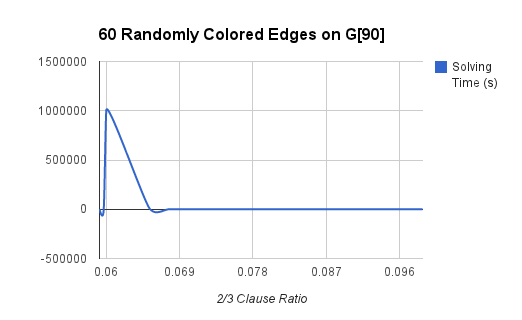
\includegraphics[scale=0.75]{chart_1.png}
\end{center}
\caption{The global maximum should lie at infinity (the solver did not finish within a time frame of 5 hours).} 
\label{f1}
\end{figure}

\begin{figure}
\begin{center}
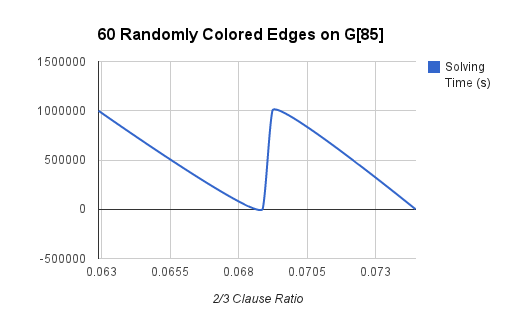
\includegraphics[scale=0.75]{chart_2.png}
\end{center}
\caption{The global maximum should lie at infinity (the solver did not finish within a time frame of 5 hours).} 
\label{f2}
\end{figure}

\begin{figure}
\begin{center}
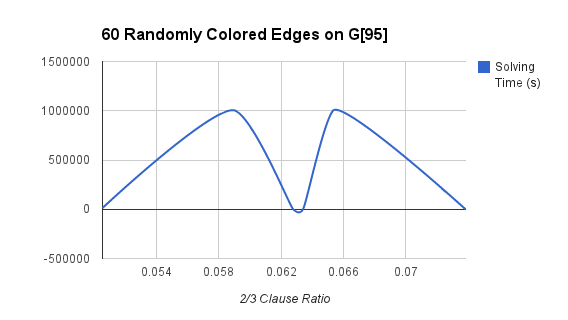
\includegraphics[scale=0.75]{chart_3.png}
\end{center}
\caption{The global maximum should lie at infinity (the solver did not finish within a time frame of 5 hours).} 
\label{f3}
\end{figure}

\begin{figure}
\begin{center}
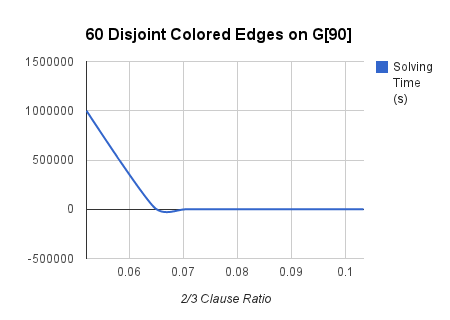
\includegraphics[scale=0.75]{chart_4.png}
\end{center}
\caption{The global maximum should lie at infinity (the solver did not finish within a time frame of 5 hours).} 
\label{f4}
\end{figure}

\begin{figure}
\begin{center}
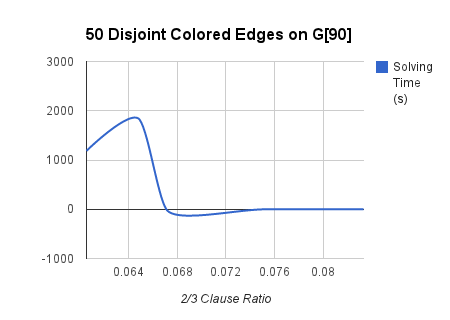
\includegraphics[scale=0.75]{chart_5.png}
\end{center}
\caption{The global maximum should lie at infinity (the solver did not finish within a time frame of 5 hours).} 
\label{f5}
\end{figure}

% \section{Exploring Other Candidate Graphs}
% While the residue graph $G_{127} = G(127,3)$ is one potential candidate for a 
% graph witnessing $G \to (3,3;4)^e$, it is natural to consider of other types of
% graphs for this property. In particular, we consider distance-based circulant graphs,
% GCD circulant graph, random graphs that are $K_4$-free, and Lu's circulant graphs
% $L(m,s)$. A typical circulant graph is defined by the pair $(\mathbb{Z}_n, \{xy : x - y \in S\})$. GCD circulant graphs are very similar, but are simply characterized
% by the fact that $E(G) = \{xy : (x,y) = 1\}$. 
% The graph $L(m,s)$, where $m$ and $s$ are relatively prime integers,
% is defined as the pair $(\mathbb{Z}_n, \{xy : x - y \in s^i \mod m \})$.

% \begin{table*}[t]
% 	\caption{SAT solver guidance experimental results for circulant graphs.}
% 	\begin{tabular}{c | c | c | c | c | c | c}
% 		\hline
% 		$n$ & $m_s$ & $m_r$ & $r$ & $V$ (min, avg, max) & $C$ (min, avg, max) & $R$ (min, avg, max) \\ \hline
% 		NA & NA & NA & NA & NA & NA & NA \\
% 		\hline
% 	\end{tabular}
% 	\label{tab:guidanceExperiment-circulant}
% \end{table*}

% \begin{table*}[t]
% 	\caption{SAT solver guidance experimental results for $L(m,s)$ circulant graphs.}
% 	\begin{tabular}{c | c | c | c | c | c | c | c}
% 		\hline
% 		$m$ & $s$ & $m_s$ & $m_r$ & $r$ & $V$ (min, avg, max) & $C$ (min, avg, max) & $R$ (min, avg, max) \\ \hline
% 		NA & NA & 0 & NA & NA & NA & NA & NA \\ 
% 		\hline
% 	\end{tabular}
% 	\label{tab:guidanceExperiment-lms}
% \end{table*}

% \begin{table*}[t]
% 	\caption{SAT solver guidance experimental results for random $K_4$-free graphs.}
% 	\begin{tabular}{c | c | c | c | c | c | c | c}
% 		\hline
% 		$n$ & $p$ & $m_s$ & $m_r$ & $r$ & $V$ (min, avg, max) & $C$ (min, avg, max) & $R$ (min, avg, max) \\ \hline
% 		NA & NA & NA & NA & NA & NA & NA & NA \\
% 		\hline
% 	\end{tabular}
% 	\label{tab:guidanceExperiment-random}
% \end{table*}

% TODO: description, picture, and rationale...
% TODO: write the code to construct these graphs.

% SAT has proven to be a very effective technique for proving the two-color Ramsey arrow
% operator for certain graphs. In this section we describe graph constructions that
% were used to generate candidate graphs for arrowing problems of interest.
% TODO: experiments with circulant graphs and $L(n,r)$ graphs, define both here.
% A circulant graph is a graph $G = (\mathbb{Z}_n, \{uv : u - v \in S\})$, where
% $S \subset \mathbb{Z}_n$ satisfying $-S = S$ and $0 \in S$. An example of such
% a graph is shown in Figure \ref{fig:circulant}.
% TODO: figure of small circulant.


\section{Arrowing Problems}
In this section we present some new results for edge Folkman numbers, some of which are improvements
upon results found in the literature.

\label{sec:arrowComputations}
\subsection{$F_e(3,5;13) = 18$}
The problem of determining if $G = K_8 + C_5 + C_5 \to (3,5)^e$ was proved by Nenov \cite{Nenov83-1}
to determine equality in the bound $F_e(3,5;13) \geq 18$. According to Kolev in 2008 \cite{Kolev08-2},
no one has been able to solve this arrowing problem. Using SAT reduction techniques, we have 
reduced this problem to an equivalent SAT formula as follows. For each triangle $xyz$ in $G$, add
$(xy + xz + yz)$ to $\phi_G$. Then, search for all other pairs of vertices $u,v$ such that $\{x,y,z,u,v\}$ is a clique
of size $5$. For all such sets of vertices, add $(\bar{xy} + \bar{xz} + \bar{xu} + \bar{xv} + \bar{yz} + \bar{yu} + \bar{yv} + \bar{zu} + \bar{zv} + \bar{uv})$
to $\phi_G$. The resulting formula has $143$ variables, each one corresponding to an edge in $G$,
and $4982$ clauses. Minisat was able to prove that this formula is unsatisfiable in 0.83s, thus
showing that $G \to (3,5)^e$, and therefore $F_e(3,5;13) = 18$.

%\subsection{What else?}
% Find other candidate graphs (dense ones!) that avoid cliques of size n and think of two-color parameters to try...

\begin{thebibliography}{9}

\bibitem{karp72} R. Karp, Reducibility among combinatorial problems, \emph{Complexity of Computer Computations, (RE Miller and JM Thatcher, eds.)} (1972), 85-103.

\bibitem{cook71-np} S. A. Cook, The Complexity of Theorem-Proving Procedures, \emph{In Proceedings of the third annual ACM symposium on Theory of computing (STOC '71)}. ACM, New York, NY, USA (1971), 151-158. DOI=10.1145/800157.805047. {\tt http://doi.acm.org/10.1145/800157.805047}

\bibitem{clrs90-algorithms} T. H. Gormen, C. E. Leiserson, R. L. Rivest, C. Stein, Introduction to Algorithms, \emph{MIT Press} \textbf{44} (1990), 97-138.

\bibitem{Radziszowski07-1} S. P. Radziszowski, X. Xu, On the Most Wanted Folkman Graph, \emph{Geocombinatiorics} \textbf{16} (4) (2007), 367-381.

\bibitem{minisat} N. S\"{o}rensson, N. E\`{e}n, Minisat v1.13 - A SAT Solver with Conflict-Clause Minimization, \emph{SAT 2005} (2005) 53.

\bibitem{zchaff} Y. Mahajan, Z. Fu, S. Malik, Zchaff2004: An Efficient SAT Solver, \emph{Theory and Applications of Satisfiability Testing}. Springer Berlin/Heidelberg (2005).

\bibitem{chaff} M. W. Moskewicz, C. F. Madigan, Y. Zhao, L. Zhang, S. Malik, Chaff: Engineering an efficient SAT solver, \emph{Proceedings of the 38th annual Design Automation Conference} ACM (2001).

\bibitem{Audemard09-1} G. Audemard, L. Simon, GLUCOSE: a solver that predicts learnt clauses quality, \emph{SAT Competition} (2009), 7-8.

\bibitem{DPLL} M. Davis, G. Logemann, and D. W. Loveland, A machine program for theorem-proving, \emph{Communications of the ACM} \textbf{5(7)} (1962), 394-397.

\bibitem{randomBalanced} Y. Boufkhad, O. Dubois, Y. Interian, B. Selman. Regular Random k-SAT: Properties of Balanced Formulas, \emph{Journal of Automated Reasoning} \textbf{35.1-3} (2005), 181-200.

\bibitem{satThreshold} Random k-SAT: Two moments suffice to cross a sharp threshold

\bibitem{Nenov83-1} N. Nenov, On the Zykov numbers and some of their applications in Ramsey theory (in Russian), \emph{Serdica} \textbf{9(2)} (1983), 161-167.

\bibitem{Kolev08-2} N. Kolev, New Upper Bound for the Edge Folkman Number $F_e(3,5;13)$, arXiv:0806.1403 (2008).

\bibitem{3satphase} D. M. Pennock, Q. F. Stout, Exploiting a theory of phase transitions in three-satisfiability problems, \emph{Ann Arbor} \textbf{1001} (1996), 48109.

\end{thebibliography}

\end{document}
